\clearpage

\documentclass[oneside,a4paper,titlepage]{article}

\usepackage{pdfpages}
\usepackage{graphicx}
\usepackage{geometry}
\usepackage{float}
\begin{document}

\section{Beskrivelse - Hvordan forløb processen i P1}
I skal beskrive jeres P1 projektproces så detaljeret som muligt. I må gerne komme ind på alle de
aspekter I finder relevante. I skal komme ind på følgende områder:

Samarbejdet i gruppen (organisering, konfliktforebyggelse og konfliktløsning)

Samarbejdet med vejlederne

Planlægning og projektstyring

læreprocessen (herunder problemorienteringens røde tråd)



Det er vigtigt at I venter med at analysere jeres erfaringer til efter at I er færdige med at beskrive
dem ! 


\section{Vurdering - Hvordan gik det}
Når I er færdige med at beskrive hvad I gjorde, skal I vurdere hvordan det gik. Med andre ord:
Hvad gik godt i P1? Hvad gik dårligt i P1? 

\section{Analyse – Hvorfor gik det som det gik?}
Dernæst skal I analysere jeres arbejdsprocesser og få klarlagt hvorfor noget gik godt mens andet gik dårligt. Med andre ord: Hvad er det for faktorer, som har indvirket på arbejdsprocesserne? 

\section{Syntese – Gode råd til P2}
Hvis jeres vurdering og analyse skal bidrage til at forbedre jeres evne til at håndtere det
problemorienterede og projektorganiserede gruppearbejde, skal I til slut konkretisere jeres erfaringer i nogle ’Gode råd’ til jer selv og jeres medstuderende. En god måde at formulere sådanne gode råd på er som en *start-stop-fortsæt*-liste, dvs. en liste med følgende tre sektioner:
– Dette vil vi begynde at gøre i P2, som vi ikke gjorde i P1 
– Dette vil vi ikke gøre i P2, som vi gjorde i P1
– Dette vil vi fortsætte med at gøre (gerne anderledes og bedre) i P2, som vi også gjorde i P1
Det er en god idé at tage ét område ad gangen og gøre det færdigt. De ’Gode råd’ skal være
konkrete og operationelle, så de fører til reelle forbedringer i P2. 


Spørgsmål til inspiration
Når I skal skrive P1-procesanalysen kan I lade jer inspirere af spørgsmålene herunder, men I må
gerne medtage andre emner, som I mener har haft betydning for jeres arbejdsprocesser.
Projektplanlægning
 Har alle i gruppen samme opfattelse af hvad projektplanlægning er ? Find ud af det.
 Har I haft en projektleder i gruppen ? Hvorfor/Hvorfor ikke ?
 Hvilke opgaver har projektledelsen i jeres projektorganisation ? (F.eks. tidsplanlægning -
ressourcefordeling - uddelegering af opgaver – motivering – kontakt udadtil - andet)
 Hvordan er de opgaver organiseret ?
 Hvilke projektplaner har I anvendt og til hvad ?
 Hvad er jeres erfaringer med projektplanerne ?
 Hvilke eksperimenter har I gennemført mht. projektplanlægning og styring ?
 Hvilke erfaringer har eksperimenterne givet jer ?
 Hvad vil I foreslå til planlægning og styring af et P2 projekt ?
Samarbejdet i gruppen
 Efter hvilke kriterier fordeler I arbejdsopgaverne mellem jer ?
 Har I en samarbejdsaftale (mundtlig / skriftlig ) ? Hvorfor/Hvorfor ikke ?
 Hvor tit holder I møder ? - Hvad hvis I kommer for sent/ikke kommer?
 Hvordan afvikles møderne ? (mødeleder ? - runde om bordet ? Andet ?)
 Har I talt om jeres forventninger til hinanden ? (F.eks. om hvad der motiverer jer,
ambitionsniveau, social deltagelse ???)
 Hvordan er kommunikationen i jeres gruppe ? Er der nogle der taler hele tiden ? Er der nogen
der aldrig siger noget ? Bruger gruppen uforholdsvis lang tid på diskussionerne ? Hvorfor ?
 Hvilke erfaringer fik I fra "Ørkenspillet", Kommunikationsdiagrammer og andre
observationer ?
 Hvad har I gjort for at udvikle jeres samarbejde i en positiv retning ?
 Hvilke eksperimenter har I gennemført i den forbindelse ?
 Hvilke forventninger har I til samarbejdet i P2 ? Hvordan skal de blive opfyldt ?
Samarbejdet med vejlederne
 Hvordan forbereder I møder med jeres vejleder ?
 Hvilken type respons ønsker I fra vejlederen ?
 Har I en samarbejdsaftale med jeres vejleder ?
 Hvilken type vejledning har I modtaget ? Var det hvad I ønskede jer ?
 Hvilke eksperimenter har I gennemført for at forbedre samarbejdet med jeres vejledere ?
 Hvad er jeres erfaringer fra de eksperimenter ?
 Hvilke forventninger vil I stille til jeres vejledere i P2 ?
Læreprocesserne
 Hvordan hjælper I hinanden med at løse opgaver i kurserne ?
 Hvad gør I hvis I ikke forstår det der bliver sagt/eller står i bogen ?
 Hvordan lærer du bedst ?
 Hvordan har I brugt resultaterne af jeres individuelle læringstest ?
 Hvordan hjælper/stimulerer vejlederen jeres læreprocesser ?
 Hvilken læringsstrategi er bedst til kurser ?
 Hvilken læringsstrategi er bedst til projektarbejde ?



\section{Bilag}

\subsection{Belbins teamroller}
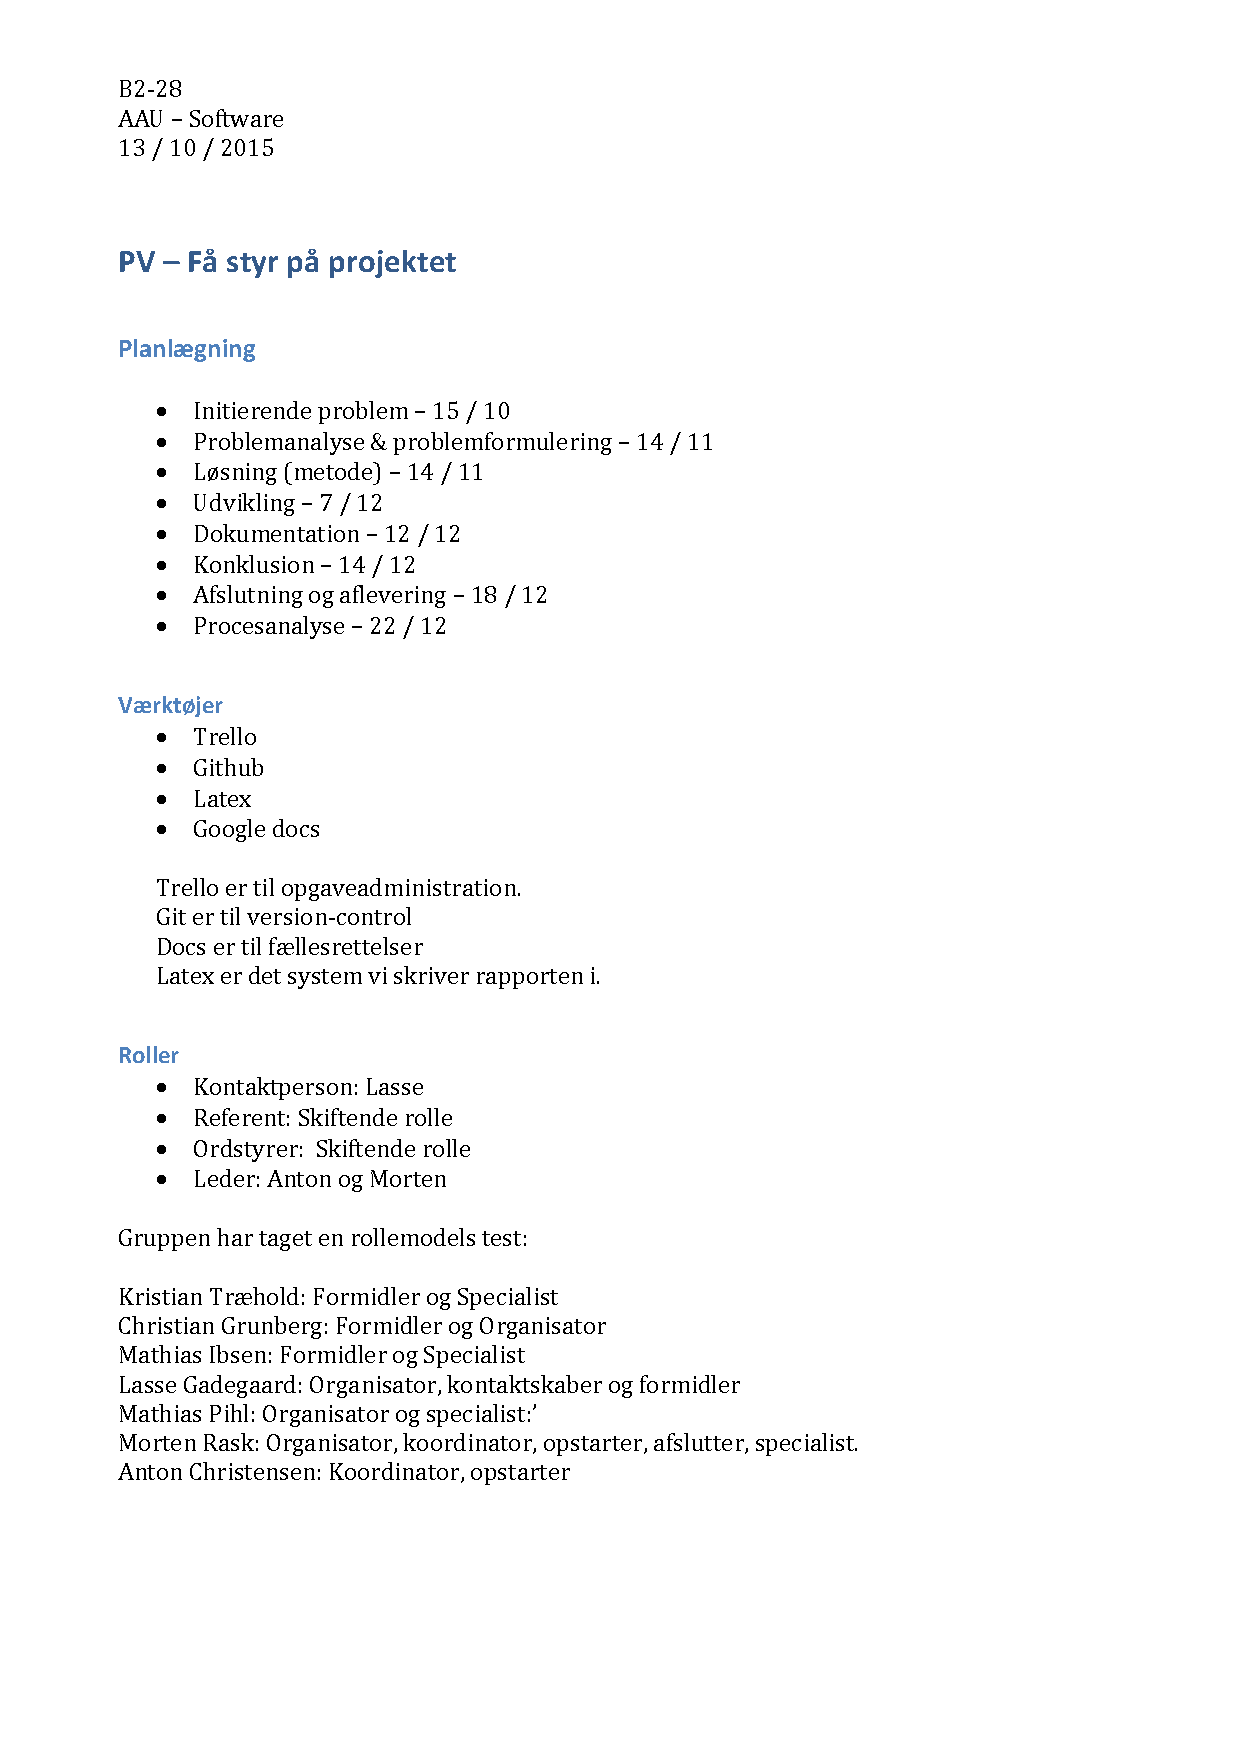
\includepdf[pages={1-2}]{../graphics/PV_bilag.pdf}
\subsection{Samarbejdsaftale mm.}
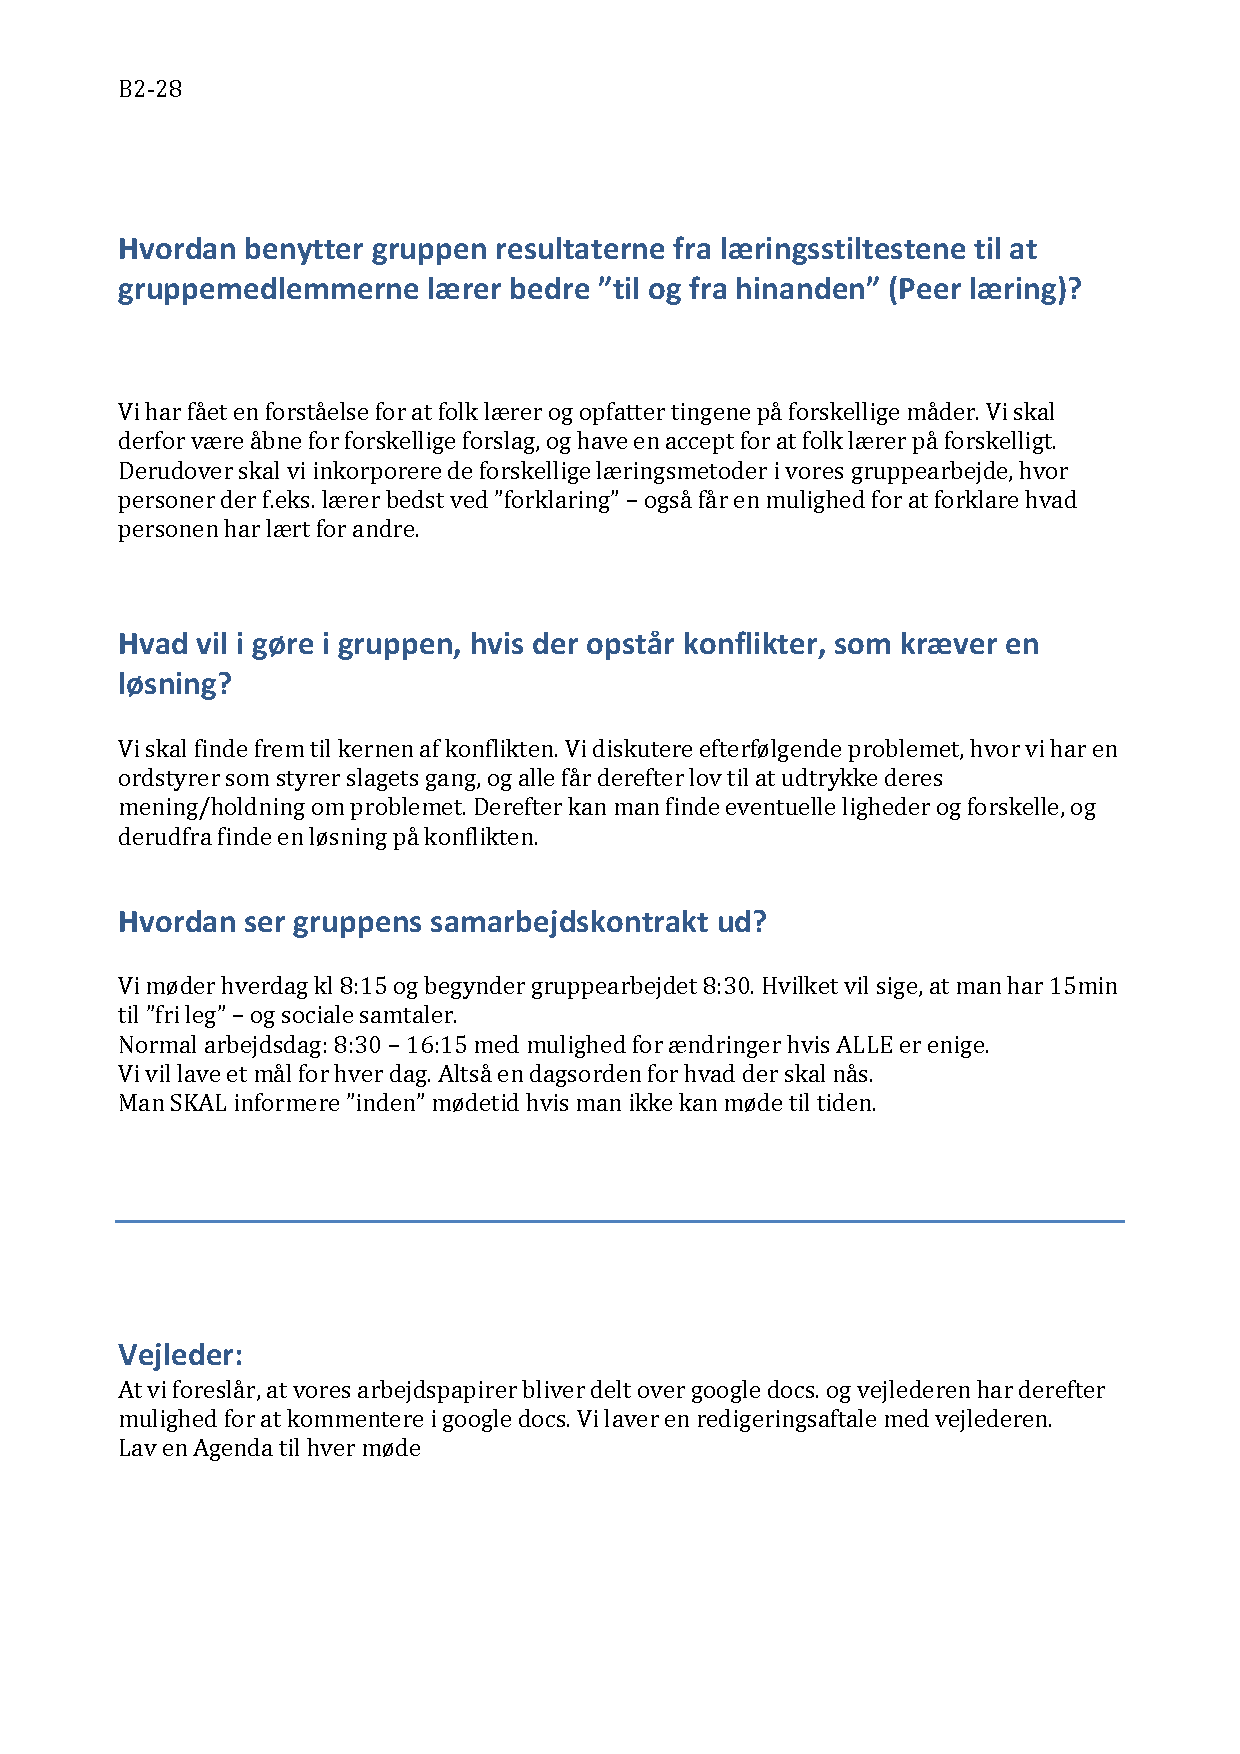
\includepdf[pages={1}]{../graphics/samarbejdsaftale_bilag.pdf}
\subsection{Mail korrespondence}
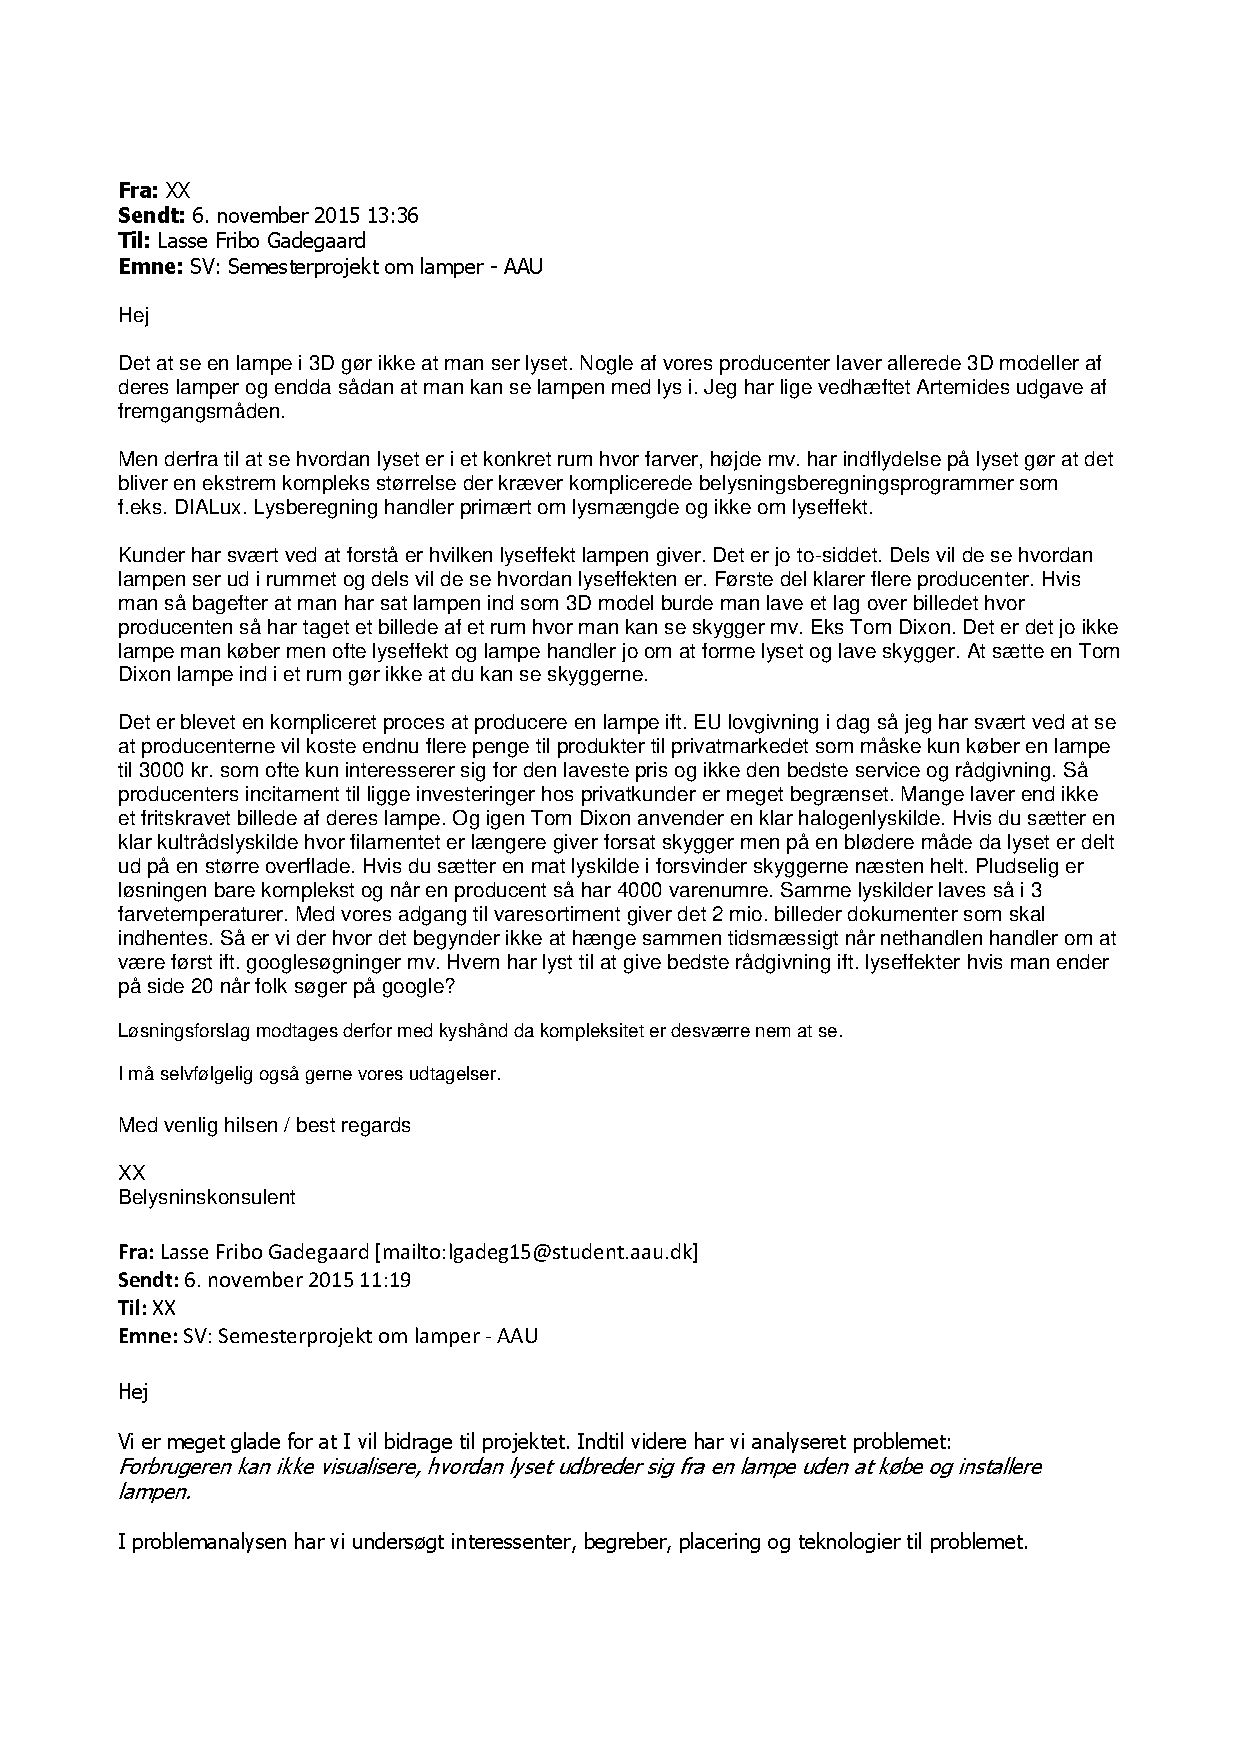
\includepdf[pages={1-3}]{../graphics/mails.pdf}

\begin{figure}[H]
   \centering
   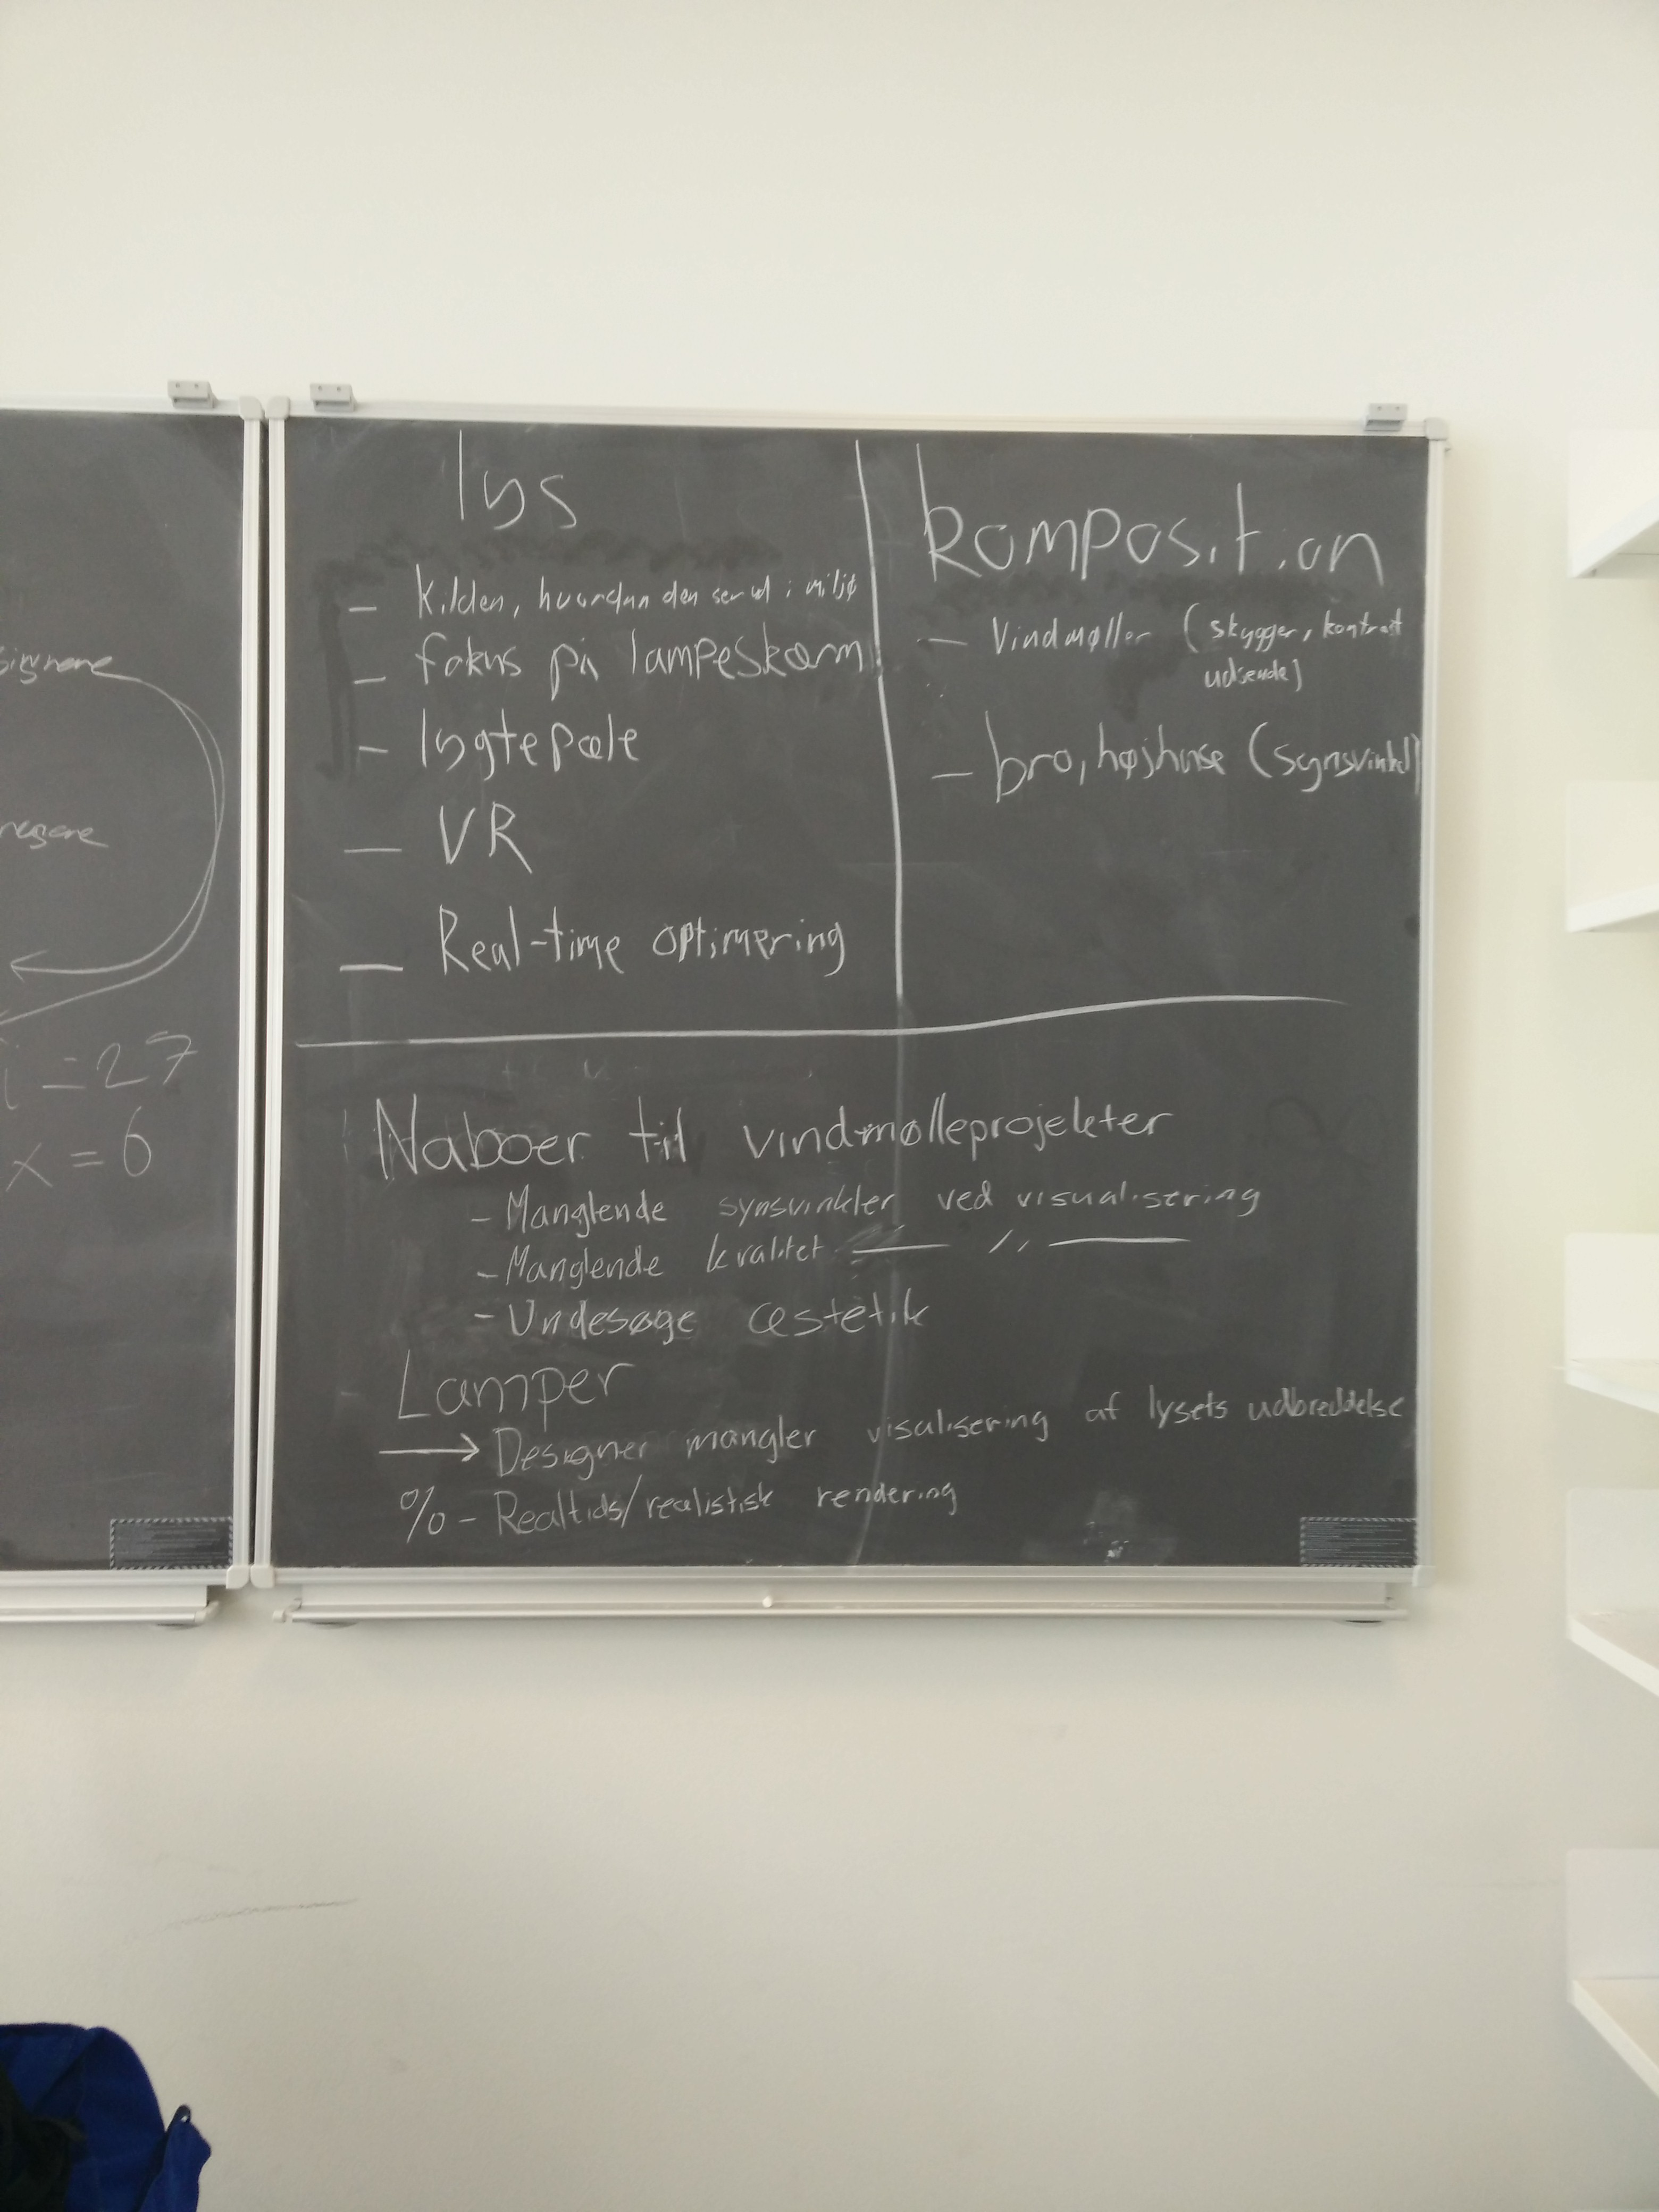
\includegraphics[width=10cm]{../graphics/brainstorm_1}
   \caption{Billede af første brainstorm}.
\end{figure}

\end{document}
